\documentclass{article}

%----------------------------------Packages------------------------------------%
\usepackage{graphicx, float}            % Graphics/Images.
\usepackage[dvipsnames]{xcolor}         % Color names.
\usepackage{pgfplots, tikz}             % Drawing/graphing tools.

\usetikzlibrary{arrows.meta}
\pgfplotsset{compat=1.9}

\title{Tikz Stuff}
\author{Ryan Maguire}
\date{\today}
\begin{document}
    \maketitle
    \section{Stick Figures}
        \begin{figure}[H]
            \centering
            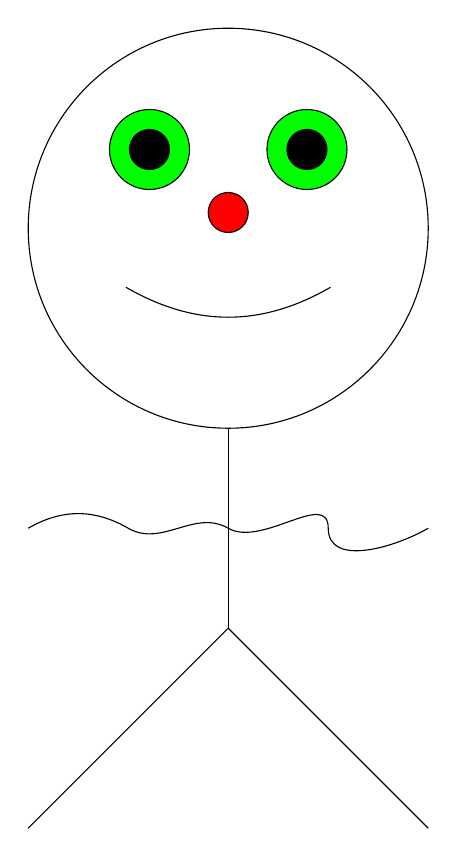
\begin{tikzpicture}
                \coordinate (Nose)      at ( 0, 0.2);
                \coordinate (Right_Eye) at ( 1, 1);
                \coordinate (Left_Eye)  at (-1, 1);
                \coordinate (Center)    at ( 0, 0);

                \coordinate (Left_Smile)  at (210:1.5);
                \coordinate (Right_Smile) at (330:1.5);

                \draw (Center) circle (1in);

                \draw[fill=green] (Right_Eye) circle (0.2in);
                \draw[fill=green] (Left_Eye)  circle (0.2in);
                \draw[fill=black] (Right_Eye) circle (0.1in);
                \draw[fill=black] (Left_Eye)  circle (0.1in);
                \draw[fill=red]   (Nose)      circle (0.1in);

                \draw (Left_Smile) to[out=-30, in=-150] (Right_Smile);
                \draw (0, -1in) to (0, -2in);
                \draw (-1in, -3in) to (0, -2in) to (1in, -3in);
                
                \draw (-1in, -1.5in) to[out=30,  in=150]  (-0.5in, -1.5in)
                                     to[out=-30, in=150]  ( 0.0in, -1.5in)
                                     to[out=-30, in=90]   ( 0.5in, -1.5in)
                                     to[out=-90, in=-150] ( 1.0in, -1.5in);
                                     
            \end{tikzpicture}
            \caption{A Stick Figure}
        \end{figure}
        \newpage
        \begin{figure}[H]
            \centering
            \begin{tikzpicture}[>=Stealth]
                \coordinate (A) at (0, 4);
                \coordinate (B) at (0, 0);
                \coordinate (C) at (-2, -4);
                \coordinate (D) at ( 2, -5);
                
                \draw[->,shorten >=0.25in]   (A) to (B);
                \draw[->, shorten >=0.40in] (B) to (0, -5);

                \draw[fill=white] (A) circle (1.2);
                \draw[fill=white] (B) ellipse (1.2 and 0.6) node {Other Thing};
                \draw[fill=white] (C) rectangle node {The End Thing} (D);

                \node (Text) at (4, 4) [below=2in] {Super cool text};
            \end{tikzpicture}
            \caption{A Flow Chart}
        \end{figure}
        
\end{document}